\documentclass[../main.tex]{subfiles}
\graphicspath{{\subfix{../images/}}}
\begin{document}


\section{Integration by parts - DI Method}
There is a nice shortcut method for integration by parts, called the DI method (DI stands for Differentiate / Integrate).

To start, set up two columns under the headings D and I. 

Then add multiple rows below them, alternating a plus (+) then minus (-) sign in front of each row:

\begin{tabular}{ c c c }
   & D & I \\ 
 + &  &  \\  
 - &  & \\
  + &  &  \\  
 - &  & \\
\end{tabular}

For an integral, we then choose which factor will go in each column. Generally, you will want to put the factor that will eventually differentiate to zero into the D column.

We then repeatedly differentiate the term in the D column, and integrate the term in the I column, until one of three possible scenarios is reached (see the three examples below).

\subsection*{Scenario 1: We get zero in the D column}
\(\int x^2 \sin{3x}\, dx\)

\begin{tabular}{ c c c }
   & D & I \\ 
 +  & $x^2$ &$\sin{3x}$ \\  
 - & $2x$ & $-\frac{\cos{3x}}{3}$\\
  + & $2$ & $-\frac{\sin{3x}}{9}$ \\  
 - & $0$ & $\frac{\cos{3x}}{27}$\\
\end{tabular}

When we reach the zero, we can stop. The integral is found by the product of the diagonals:
\begin{figure}[h]
    
    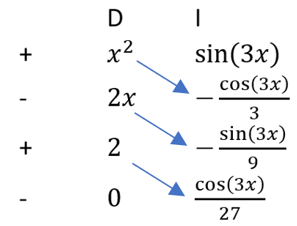
\includegraphics[width=0.22\linewidth]{images/dimethod1.png}
\end{figure}

This is where the signs out the front of each row are key. When we calculate the product of each diagonal, the sign tells us whether to add or subtract that product.

In this example, the integral will be:

\(x^2 \times -\frac{\cos{3x}}{3}-2x\times -\frac{\sin{3x}}{9}+2\times \frac{\cos{3x}}{27}+c\)

\(=-\frac{x^2\cos{3x}}{3}+\frac{2x\sin{3x}}{9}+\frac{2\cos{3x}}{27}+c\)

\subsection*{Scenario 2: When we can integrate the product of a row}
\(\int x^4 \ln{x}\, dx\)

Firstly, notice that we put the l\(\ln{x}\) in the D column as we would need to integrate it by parts.

\begin{tabular}{ c c c }
   & D & I \\ 
 +  & $\ln{x}$ &$x^4$ \\  
 - & $\frac{1}{x}$ & $\frac{x^5}{5}$\\
\end{tabular}

We can now stop at the second row as the product \(\frac{x^4}{5}\) can be easily integrated. 

The integral is now found by the product(s) of the diagonals as in the previous example, but we also need to take into account the final row. We add/subtract (based on the sign of the row) the integral of the product of this final row.
\begin{figure}[h]
    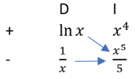
\includegraphics{images/dimethod2.png}
\end{figure}

The integral will therefore be:

\(\ln{x} \times \frac{x^5}{5}-\int \frac{1}{x}\times \frac{x^5}{5}\, dx\)

\(=\frac{x^5}{5}\ln{x}-\frac{x^5}{25}+c\)

\subsection*{Scenario 3: When a row “repeats”}
\(\int e^x \sin{x}\,dx\)

Since we can easily integrate both factors, it doesn’t matter which one we put in the I column. In this example we will put \(\sin{x}\) there.

\begin{tabular}{ c c c }
   & D & I \\ 
 +  & $e^x$ &$\sin{x}$ \\  
 - & $e^x$ & $-\cos{x}$\\
  + & $e^x$ & $-\sin{x}$ \\  
\end{tabular}

Notice how the third row has the same terms in it. This means we can stop.

As in scenario 2, we find the integral by taking the products of the diagonals and then adding/subtracting the integral of the product of the final row.

\begin{figure}[h]
    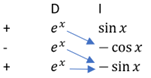
\includegraphics{images/dimethod3.png}
\end{figure}

The integral will be:

\(-e^x\cos{x}+e^x\sin{x}+\int -e^x\sin{x}\,dx\)

We can now form an equation for our integral:

\(\int e^x \sin{x}\,dx=-e^x\cos{x}+e^x\sin{x}-\int e^x\sin{x}\,dx\)

Rearranging and solving:

\(2\int e^x \sin{x}\,dx=-e^x\cos{x}+e^x\sin{x}\)

\(\int e^x \sin{x}\, dx=\frac{-e^x\cos{x}+e^x\sin{x}}{2}\)

\pagebreak

\subsection*{Questions}
\label{DI Method}
\begin{enumerate}
    \item \(\int x^2\sin{(2x)}\, dx\)

    \item \(\int e^x \cos{(x)}\, dx\)

    \item \(\int (\ln{(x)})^2\, dx\)

    \item \(\int \sin^3{(x)}\,dx\)

    \item \(\int \frac{\ln{(x)}}{x^2}\, dx\)

    \item \(\int 4x\cos{(2-3x)}\, dx\)

    \item \(\int e^{-x}\cos{(x)}\, dx\)

    
\end{enumerate}


\pagebreak


\end{document}